\subsection{Active levitation (parameters validation)}
\label{subsec:active_levitation}

\textit{
    For the sake of identification, we ignore here for a moment the description of the controller used to perform the active control on the ball position given that in Section \ref{subsubsec:pid_anti_windup} we will describe the controller in detail.
}

The final step of the identification process is to perform an active levitation test to check that the electromagnetic force predicted by the coefficients retrieved in Section \ref{subsec:inductances_characterization} and Section \ref{subsec:force_analysis} is accurate.
This test is crucial to validate the overall model and to obtain the final values of the coefficients.

The active levitation test consists of applying a control signal to the coils to maintain the ball at a fixed position.
Performing the test at different ball heights and annotating the corresponding current values allows us to determine experimentally the relationship $I_{op} = I_{op}(z_{op})$.
As we have already seen in Section \ref{subsec:model_linearization}, the relationship between the current and the ball position is given by:

\begin{equation}
    I_{op} = \sqrt{ - \left(2m g + \frac{\partial L_2}{\partial z} \big|_{z_{op}} (\frac{V_{2min}}{R_{20}})^2 \right) / \frac{\partial L_1}{\partial z} \big|_{z_{op}} } \approx \sqrt{ - \left(2m g \right) / \frac{\partial L_1}{\partial z} \big|_{z_{op}} }
    \label{eq:current_position_relation}
\end{equation}

In the left-hand side of Figure \ref{fig:active_levitation} we show the time evolution of the ball position during the active levitation test.
One can easily see that the ball is maintained at three different heights by applying different control signals to the coils.

Instead, in the right-hand side of Figure \ref{fig:active_levitation}, the experimentally determined operating points, their interpolation and the theoretical curve given by Equation \ref{eq:current_position_relation} using the coefficients listed in Table \ref{tab:inductance_characterization_parameters} are shown.

\begin{figure}[H]
    \centering
    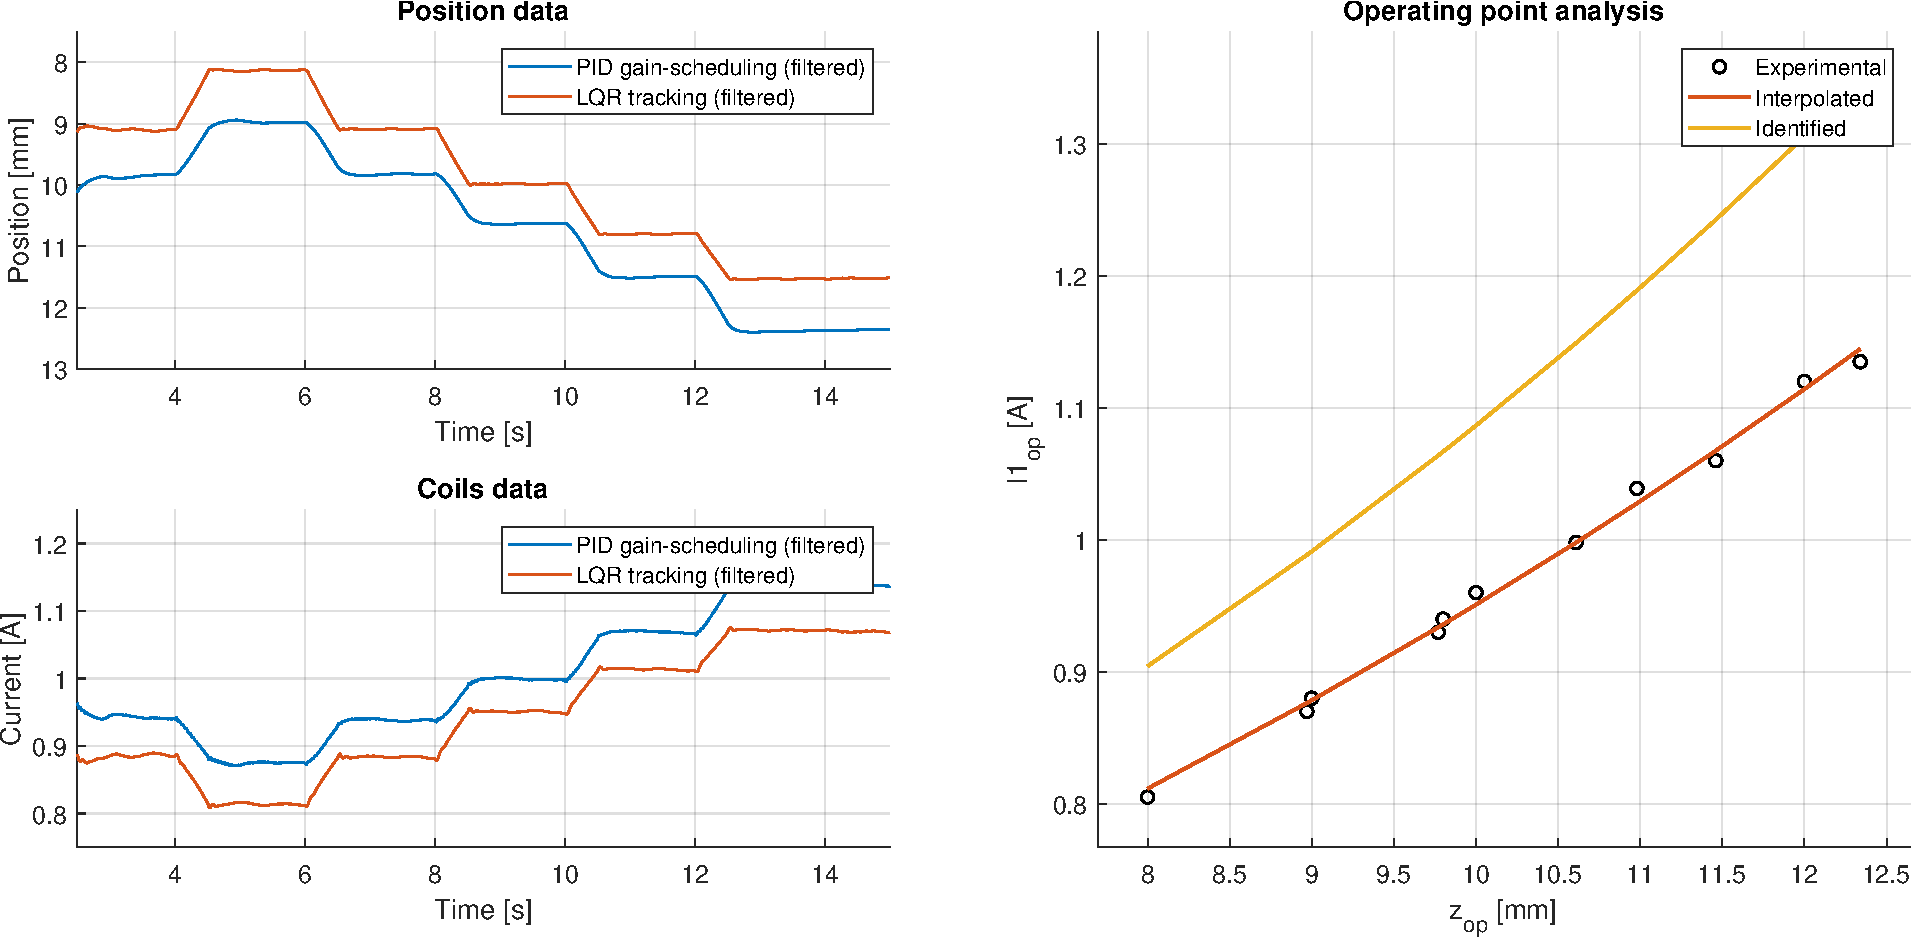
\includegraphics[width=1\textwidth]{img/MATLAB/identification/operating_point_analysis.pdf}
    \caption{Comparison of the operating point between the theoretical model and the experimental data obtained during the active levitation test.}
    \label{fig:active_levitation}
\end{figure}

As we can see, the curve based on the parameters of Table \ref{tab:inductance_characterization_parameters} doesn't fit the experimental data as expected.
The gap between the identified and the theoretical curve, might found its origin in the assumption of neglecting the term $\frac{\partial L}{\partial I} I$ in Equation \ref{eq:voltage_in_rl_circuit} when fitting the current dynamics in Section \ref{subsec:inductances_characterization} or due to poor identification of the levitation point in case of the procedure followed in Section \ref{subsec:force_analysis}.

In any case, given the large distance between the theoretical curve and the experimental data, we decided to discard the previously identified parameters and to re-identify them using the data obtained from the active levitation test which is considered more reliable.

The final values of the parameters are shown in Table \ref{tab:final_inductance_characterization_parameters}.

\begin{table}[H]
    \centering
    \begin{tabular}{|c|c|c|}
        \hline
        \textbf{Parameter} & \textbf{Value}           & \textbf{Units} \\
        \hline
        $L_0$              & $6.539244 \cdot 10^{-2}$ & $H$            \\
        $a_z$              & $1.585423 \cdot 10^{+2}$ & $1/m$          \\
        $L_z$              & $4.044743 \cdot 10^{-2}$ & $H$            \\
        $a_I$              & $5.296552 \cdot 10^{+0}$ &                \\
        $b_I$              & $1.042271 \cdot 10^{+0}$ & $A$            \\
        $L_I$              & $3.288792 \cdot 10^{-2}$ & $H$            \\
        \hline
    \end{tabular}

    \caption{Final inductance parameters obtained via active levitation test.}
    \label{tab:final_inductance_characterization_parameters}

\end{table}

Notice that with respect to the values presented in Table \ref{tab:inductance_characterization_parameters}, only $a_z$ and $L_z$ have been directly obtained from the active levitation test.
All the others have been re-identified by keeping fixed the values of $a_z$ and $L_z$ and by re-fitting the inductance model to the experimental data of currents dynamics as already described in Section \ref{subsec:inductances_characterization}.



